%%%%%%%%%%%%%%%%%%%%%%%%%%%%%%%%%%%%%%%%%
% Beamer Presentation
% LaTeX Template
% Version 1.0 (10/11/12)
%
% This template has been downloaded from:
% http://www.LaTeXTemplates.com
%
% License:
% CC BY-NC-SA 3.0 (http://creativecommons.org/licenses/by-nc-sa/3.0/)
%
%%%%%%%%%%%%%%%%%%%%%%%%%%%%%%%%%%%%%%%%%

%----------------------------------------------------------------------------------------
%	PACKAGES AND THEMES
%----------------------------------------------------------------------------------------

\documentclass[9pt]{beamer}
\usepackage{CJK}
\usepackage{ctex}
\usepackage{graphicx}
\usepackage{subfigure}
\usepackage{longtable}
\usepackage{rotating}
\usepackage{multirow}
\usepackage{algorithm}
\usepackage{algorithmic}
\usepackage{mathtools}
\usepackage{animate}
\usepackage{array}
%\usepackage{media9}
%% A LATEX package for embedding interactive Adobe Flash (SWF) and 3D files (Adobe U3D & PRC) as well as video and sound files or streams (FLV, MP4/H.246, MP3) into PDF documents with Adobe Reader-9/X
%compatibility.
\renewcommand{\algorithmicrequire}{\textbf{Input:}}   %Use Input in the format of Algorithm
\renewcommand{\algorithmicensure}{\textbf{Output:}}  %UseOutput in the format of Algorithm
\newcommand{\e}[1]{\ensuremath{\times 10^{#1}}}
%\mode<presentation>{\usetheme{Madrid}}

\mode<presentation> {

% The Beamer class comes with a number of default slide themes
% which change the colors and layouts of slides. Below this is a list
% of all the themes, uncomment each in turn to see what they look like.

%\usetheme{default}
%\usetheme{AnnArbor}
%\usetheme{Antibes}
%\usetheme{Bergen}
%\usetheme{Berkeley}
%\usetheme{Berlin}
%\usetheme{Boadilla}
%\usetheme{CambridgeUS}
%\usetheme{Copenhagen}
%\usetheme{Darmstadt}
%\usetheme{Dresden}
%\usetheme{Frankfurt}
%\usetheme{Goettingen}
%\usetheme{Hannover}
%\usetheme{Ilmenau}
%\usetheme{JuanLesPins}
%\usetheme{Luebeck}
\usetheme{Madrid}
%\usetheme{Malmoe}
%\usetheme{Marburg}
%\usetheme{Montpellier}
%\usetheme{PaloAlto}
%\usetheme{Pittsburgh}
%\usetheme{Rochester}
%\usetheme{Singapore}
%\usetheme{Szeged}
%\usetheme{Warsaw}

% As well as themes, the Beamer class has a number of color themes
% for any slide theme. Uncomment each of these in turn to see how it
% changes the colors of your current slide theme.

%\usecolortheme{albatross}
\usecolortheme{beaver}
%\usecolortheme{beetle}
%\usecolortheme{crane}
%\usecolortheme{dolphin}
%\usecolortheme{dove}
%\usecolortheme{fly}
%\usecolortheme{lily}
%\usecolortheme{orchid}
%\usecolortheme{rose}
%\usecolortheme{seagull}
%\usecolortheme{seahorse}
%\usecolortheme{whale}
%\usecolortheme{wolverine}

%\setbeamertemplate{footline} % To remove the footer line in all slides uncomment this line
%\setbeamertemplate{footline}[page number] % To replace the footer line in all slides with a simple slide count uncomment this line

%\setbeamertemplate{navigation symbols}{} % To remove the navigation symbols from the bottom of all slides uncomment this line
}

\usepackage{graphicx} % Allows including images
\usepackage{booktabs} % Allows the use of \toprule, \midrule and \bottomrule in tables
\begin{document}
\begin{CJK*}{GBK}{kai}
%----------------------------------------------------------------------------------------
%	TITLE PAGE
%----------------------------------------------------------------------------------------

\title[Machine Learning]{LN13. ~~Bias Variance Tradeoff} % The short title appears at the bottom of every slide, the full title is only on the title page

\author{Kun He (����)} % Your name
%\logo{%
%   
\includegraphics[scale=.2]{logo.pdf}\hspace*{4.75cm}~%
%   
\includegraphics[scale=.2]{logo.jpg}\hspace*{0.75cm}%
%   }
%\pgfdeclareimage[width=1cm]{hust}{logo.pdf}
%\logo{\pgfuseimage{hust}{\vspace{-10pt}}}
\titlegraphic{
\includegraphics[width=1.3cm]{logo.pdf}}
\institute[JHL, HUST] % Your institution as it will appear on the bottom of every slide, may be shorthand to save space
{
	Data Mining and Machine Learning Lab\\
	(John Hopcroft Lab)\\
	Huazhong University of Science \& Technology \\ % Your institution for the title page
	\medskip
	\textit{brooklet60@hust.edu.cn} % Your email address
}

\date{2022��5��} % Date, can be changed to a custom date
%====================================================
\frame{\titlepage}

\frame{\frametitle{Table of Contents}\tableofcontents}

\AtBeginSection[]
{
	\begin{frame}{Table of Contents}
		\tableofcontents[currentsection]
	\end{frame}
}


%------------------------------------------------
%------------------------------------------------
%------------------------------------------------
\section{Concept}
%------------------------------------------------
\subsection{Problem Settings}
\begin{frame}
	\frametitle{Assumptions}
	\begin{block}{Assumptions}
		\begin{itemize}
			\item
			As usual, we are given a dataset $D={(\mathbf{x}_1,y_1),��,(\mathbf{x}_n,y_n)}$, drawn i.i.d. from some distribution $P(X,Y)$.
			\item
			Throughout this lecture we assume a regression setting, i.e. $y\in \mathbb{R}$. 
		\end{itemize}
	\end{block}
\end{frame}

\begin{frame}
	\frametitle{Purpose}
	\begin{block}{Purpose}
		In this lecture we will decompose the generalization error of a classifier into three rather interpretable terms.
	\end{block}
\end{frame}

\subsection{Preliminary}

\begin{frame}
	\frametitle{Preliminary}
	\begin{block}{Preliminary}
	Before we do that, let us consider that for any given input $\mathbf{x}$ there might not exist a unique label $y$. For example, if your vector $\mathbf{x}$ describes features of house (e.g. \#bedrooms, square footage, ...) and the label $y$ its price, you could imagine two houses with identical description selling for different prices.
	\\~~\\So for any given feature vector $\mathbf{x}$, there is a distribution over possible labels. We therefore define the following, which will come in useful later on:
	\end{block}
\end{frame}

\begin{frame}
	\frametitle{Expected Label}
	\begin{block}{\textbf{Expected Label}~(given $\mathbf{x} \in \mathbb{R}^d$)}
		\begin{center}
			$\bar{y}(\mathbf{x})=E_{y \mid \mathbf{x}}[Y]=\int_{y} y \operatorname{Pr}(y \mid \mathbf{x}) \partial y .$
		\end{center}
		The expected label denotes the label you would expect to obtain, given a feature vector $\mathbf{x}$. 
	\end{block}
\end{frame}

\begin{frame}
	\frametitle{Expected Test Error}
	
	Alright, so we draw our training set $D$, consisting of $n$ inputs, i.i.d. from the distribution $P$. As a second step we typically call some machine learning algorithm $\mathcal{A}$ on this data set to learn a hypothesis (aka classifier). Formally, we denote this process as $h_D = \mathcal{A}(D)$.
	
	For a given $h_D$, learned on data set $D$ with algorithm $\mathcal{A}$, we can compute the generalization error (as measured in squared loss) as follows:
	
\end{frame}

\begin{frame}
	\frametitle{Expected Test Error}
	\begin{block}{\textbf{Expected Test Error}~(given $h_D$)}
		\begin{center}
			$E_{(\mathbf{x}, y) \sim P}\left[\left(h_{D}(\mathbf{x})-y\right)^{2}\right]=\int_{\mathbf{x}}\int_y\left(h_{D}(\mathbf{x})-y\right)^{2} \operatorname{Pr}(\mathbf{x}, y) \partial y \partial \mathbf{x} .$
		\end{center}
		Note that one can use other loss functions. We use squared loss because it has nice mathematical properties, and it is also the most common loss function.
	\end{block}
\end{frame}

\begin{frame}
	\frametitle{Expected Classifier}
	The previous statement is true for a given training set $D$. However, remember that $D$ itself is drawn from $P^n$, and is therefore a random variable. Further, $h_D$ is a function of $D$, and is therefore also a random variable. And we can of course compute its expectation:
\end{frame}

\begin{frame}
	\frametitle{Expected Classifier}
	\begin{block}{\textbf{Expected Classifier}~(given $\mathcal{A}$)}
		\begin{center}
			$\bar{h}=E_{D \sim P^{n}}\left[h_{D}\right]=\int_{D} h_{D} \operatorname{Pr}(D) \partial D .$
		\end{center}
		where $\operatorname{Pr}(D)$ is the probability of drawing $D$ from $P^n$. Here, $\bar{h}$ is a weighted average over functions.
	\end{block}
\end{frame}

\begin{frame}
	\frametitle{Expected Test Error}
	We can also use the fact that $h_D$ is a random variable to compute the expected test error only given $\mathcal{A}$, taking the expectation also over $D$.
\end{frame}

\begin{frame}
	\frametitle{Expected Test Error}
	\begin{block}{\textbf{Expected Test Error}~(given $\mathcal{A}$)}
		\begin{center}
			$\underset{(\mathbf{x}, y) \sim P \atop D \sim P^{n}}{E}\left[\left(h_{D}(\mathbf{x})-y\right)^{2}\right]=\int_{D} \int_{\mathbf{x}} \int_{y}\left(h_{D}(\mathbf{x})-y\right)^{2} \mathrm{P}(\mathbf{x}, y) \mathrm{P}(D) \partial \mathbf{x} \partial y \partial D .$
		\end{center}
		To be clear, $D$ is our training points and the $(\mathbf{x},y)$ pairs are the test points.
	\end{block}
\end{frame}

\begin{frame}{Expected Test Error}
	We are interested in exactly this expression, because it evaluates the quality of a machine learning algorithm $\mathcal{A}$ with respect to a data distribution $P(X,Y)$. 
	
	In the following we will show that this expression decomposes into three meaningful terms.
	
\end{frame}



\section{Decomposition of Expected Test Error}
\subsection{Decomposition of Expected Test Error}
\begin{frame}
	\frametitle{Decomposition of Expected Test Error}
	\begin{center}
		$
		\begin{aligned}
		&E_{\mathbf{x}, y, D}\left[\left[h_{D}(\mathbf{x})-y\right]^{2}\right] \\ =&E_{\mathbf{x}, y, D}\left[\left[\left(h_{D}(\mathbf{x})-\bar{h}(\mathbf{x})\right)+(\bar{h}(\mathbf{x})-y)\right]^{2}\right] \\
		=&E_{\mathbf{x}, D}\left[\left(\bar{h}_{D}(\mathbf{x})-\bar{h}(\mathbf{x})\right)^{2}\right]+2 E_{\mathbf{x}, y, D}\left[\left(h_{D}(\mathbf{x})-\bar{h}(\mathbf{x})\right)(\bar{h}(\mathbf{x})-y)\right]+E_{\mathbf{x}, y}\left[(\bar{h}(\mathbf{x})-y)^{2}\right]
		\end{aligned}    
		$
	\end{center}
\end{frame}


\begin{frame}
	\frametitle{Decomposition of Expected Test Error}
	The middle term of the equation is 0 as we show below
	\begin{center}
		$
		\begin{aligned}
		E_{\mathbf{x}, y, D}\left[\left(h_{D}(\mathbf{x})-\bar{h}(\mathbf{x})\right)(\bar{h}(\mathbf{x})-y)\right] &=E_{\mathbf{x}, y}\left[E_{D}\left[h_{D}(\mathbf{x})-\bar{h}(\mathbf{x})\right](\bar{h}(\mathbf{x})-y)\right] \\
		&=E_{\mathbf{x}, y}\left[\left(E_{D}\left[h_{D}(\mathbf{x})\right]-\bar{h}(\mathbf{x})\right)(\bar{h}(\mathbf{x})-y)\right] \\
		&=E_{\mathbf{x}, y}[(\bar{h}(\mathbf{x})-\bar{h}(\mathbf{x}))(\bar{h}(\mathbf{x})-y)] \\
		&=E_{\mathbf{x}, y}[0] \\
		&=0
		\end{aligned}    
		$
	\end{center}
\end{frame}


\begin{frame}
	\frametitle{Decomposition of Expected Test Error}
	Returning to the earlier expression, we're left with the variance and another term
	\begin{center}
		$
		\begin{aligned}
		E_{\mathbf{x}, y, D}\left[\left(h_{D}(\mathbf{x})-y\right)^{2}\right]=\underbrace{E_{\mathbf{x}, D}\left[\left(h_{D}(\mathbf{x})-\bar{h}(\mathbf{x})\right)^{2}\right]}_{\text {Variance }}+E_{\mathbf{x}, y}\left[(\bar{h}(\mathbf{x})-y)^{2}\right]
		\end{aligned}
		$
	\end{center}
\end{frame}


\begin{frame}
	\frametitle{Decomposition of Expected Test Error}
	We can break down the second term in the above equation as follows:
	\begin{center}
		$
		\begin{aligned}
		E_{\mathbf{x}, y}\left[(\bar{h}(\mathbf{x})-y)^{2}\right] &=E_{\mathbf{x}, y}\left[(\bar{h}(\mathbf{x})-\bar{y}(\mathbf{x}))+(\bar{y}(\mathbf{x})-y)^{2}\right] \\
		&=\underbrace{E_{\mathbf{x}, y}\left[(\bar{y}(\mathbf{x})-y)^{2}\right]}_{\text {Noise }}+\underbrace{E_{\mathbf{x}}\left[(\bar{h}(\mathbf{x})-\bar{y}(\mathbf{x}))^{2}\right]}_{\text {Bias }^{2}}+2 E_{\mathbf{x}, y}[(\bar{h}(\mathbf{x})-\bar{y}(\mathbf{x}))(\bar{y}(\mathbf{x})-y)]
		\end{aligned}
		$
	\end{center}
\end{frame}


\begin{frame}
	\frametitle{Decomposition of Expected Test Error}
	The third term in the equation above is 0, as we show below
	\begin{center}
		$
		\begin{aligned}
		E_{\mathbf{x}, y}[(\bar{h}(\mathbf{x})-\bar{y}(\mathbf{x}))(\bar{y}(\mathbf{x})-y)] &=E_{\mathbf{x}}\left[E_{y \mid \mathbf{x}}[\bar{y}(\mathbf{x})-y](\bar{h}(\mathbf{x})-\bar{y}(\mathbf{x}))\right] \\
		&=E_{\mathbf{x}}\left[E_{y \mid \mathbf{x}}[\bar{y}(\mathbf{x})-y](\bar{h}(\mathbf{x})-\bar{y}(\mathbf{x}))\right] \\
		&=E_{\mathbf{x}}\left[\left(\bar{y}(\mathbf{x})-E_{y \mid \mathbf{x}}[y]\right)(\bar{h}(\mathbf{x})-\bar{y}(\mathbf{x}))\right] \\
		&=E_{\mathbf{x}}[(\bar{y}(\mathbf{x})-\bar{y}(\mathbf{x}))(\bar{h}(\mathbf{x})-\bar{y}(\mathbf{x}))] \\
		&=E_{\mathbf{x}}[0] \\
		&=0
		\end{aligned}
		$
	\end{center}
\end{frame}


\begin{frame}
	\frametitle{Decomposition of Expected Test Error}
	\begin{block}{Decomposition of Expected Test Error}
		This gives us the decomposition of expected test error as follows
		\begin{center}
			$\underbrace{E_{\mathbf{x}, y, D}\left[\left(h_{D}(\mathbf{x})-y\right)^{2}\right]}_{\text {Expected Test Error }}=\underbrace{E_{\mathbf{x}, D}\left[\left(h_{D}(\mathbf{x})-\bar{h}(\mathbf{x})\right)^{2}\right]}_{\text {Variance }}+\underbrace{E_{\mathbf{x}, y}\left[(\bar{y}(\mathbf{x})-y)^{2}\right]}_{\text {Noise }}+\underbrace{E_{\mathbf{x}}\left[(\bar{h}(\mathbf{x})-\bar{y}(\mathbf{x}))^{2}\right]}_{\text {Bias }^{2}}$    
		\end{center}
	\end{block}
\end{frame}




\subsection{Variance, Bias and Noise}
\begin{frame}{Variance}
	\begin{block}{Variance}
		\begin{itemize}
			\item 
			Captures how much your classifier changes if you train on a different training set.
			\item
			How "over-specialized" is your classifier to a particular training set (overfitting)?
			\item
			If we have the best possible model for our training data, how far off are we from the average classifier?
		\end{itemize}
	\end{block}
\end{frame}

\begin{frame}{Bias}
	\begin{block}{Bias}
		\begin{itemize}
			\item 
			What is the inherent error that you obtain from your classifier even with infinite training data?
			\item
			This is due to your classifier being "biased" to a particular kind of solution (e.g. linear classifier).
			\item
			In other words, bias is inherent to your model.
		\end{itemize}
	\end{block}
\end{frame}

\begin{frame}{Noise}
	\begin{block}{Noise}
		\begin{itemize}
			\item 
			How big is the data-intrinsic noise?
			\item
			This error measures ambiguity due to your data distribution and feature representation.
			\item
			You can never beat this, it is an aspect of the data.
		\end{itemize}
	\end{block}
\end{frame}


\begin{frame}{Graphical illustration of bias and variance.}
	\begin{figure}[h]
		\centering
		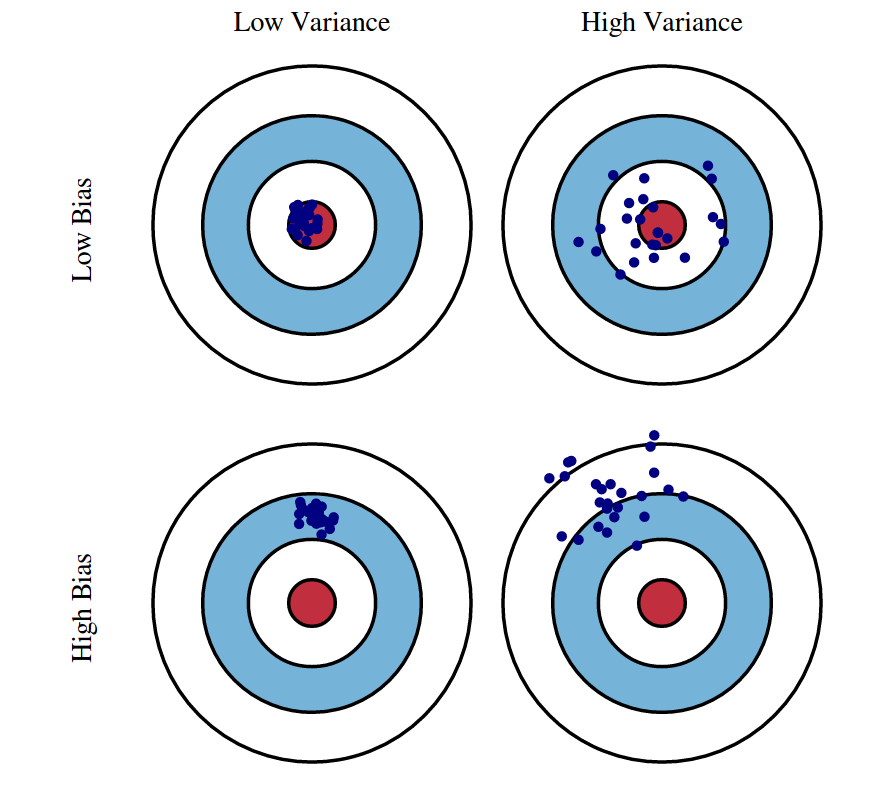
\includegraphics[scale=0.25]{pics/bullseye.png}
	\end{figure}
\end{frame}

\begin{frame}{The variation of Bias and Variance with the model complexity.}
	\begin{figure}[h]
		\centering
		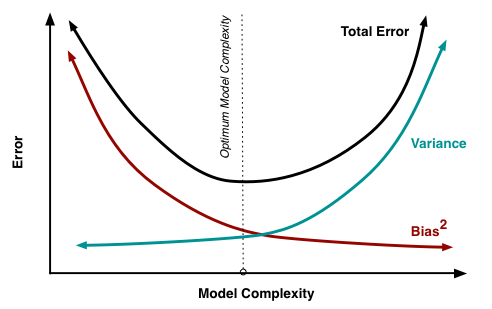
\includegraphics[scale=0.5]{pics/biasvariance.png}
	\end{figure}
	\textbf{The variation of Bias and Variance with the model complexity.} This is similar to the concept of overfitting and underfitting. More complex models overfit while the simplest models underfit.
\end{frame}


\section{Detecting High Bias and High Variance}
\subsection{How to Debug ML Algorithms}
\begin{frame}{How to Debug ML Algorithms}
	If a classifier is under-performing (e.g. if the test or training error is too high), there are several ways to improve performance. To find out which of these many techniques is the right one for the situation, the first step is to determine the root of the problem.
\end{frame}

\begin{frame}{Training and Test Error}
	\begin{figure}[h]
		\centering
		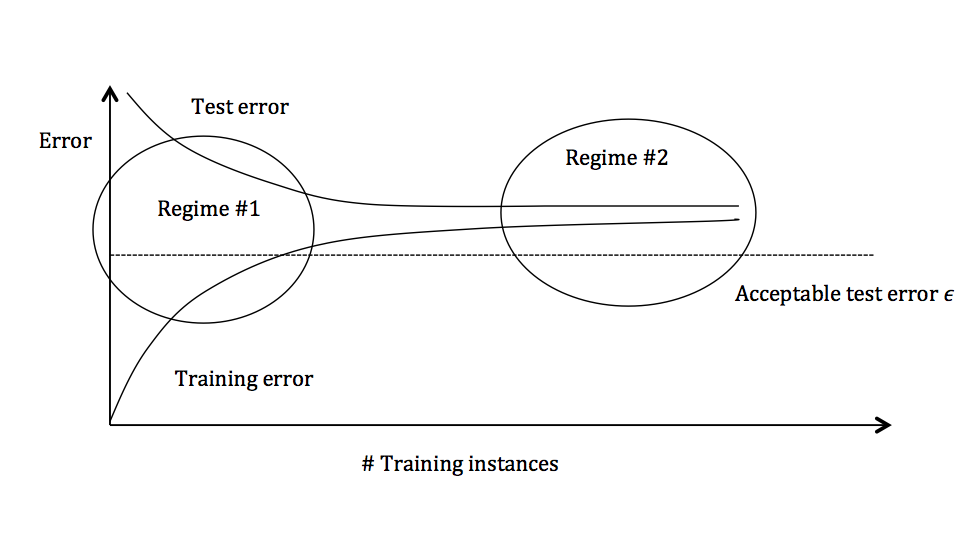
\includegraphics[scale=0.3]{pics/error.png}
	\end{figure}
	\centering
	Test and training error as the number of training instances increases.
\end{frame}

\begin{frame}{Training and Test Error}
	\begin{figure}[h]
		\centering
		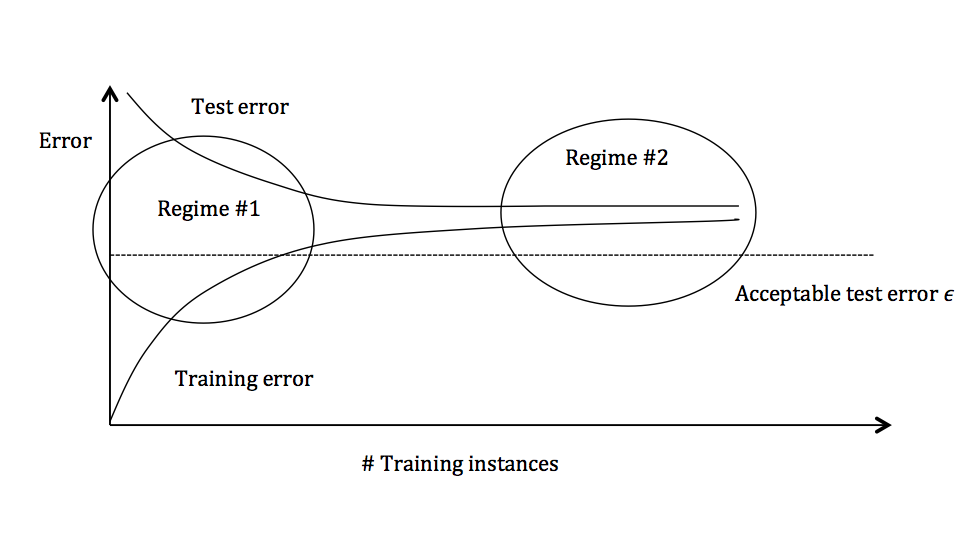
\includegraphics[scale=0.2]{pics/error.png}
	\end{figure}
	The graph above plots the training error and the test error and can be divided into two overarching regimes. 
	\begin{itemize}
		\item 
		In the first regime (on the left side of the graph), training error is below the desired error threshold (denoted by $\epsilon$), but test error is significantly higher.
		\item
		In the second regime (on the right side of the graph), test error is remarkably close to training error, but both are above the desired tolerance of $\epsilon$.
	\end{itemize}
\end{frame}


\subsection{High Variance}
\begin{frame}{Regime 1 (High Variance)}
	\begin{block}{Regime 1 (High Variance)}
		In the first regime, the cause of the poor performance is high variance.
	\end{block}
\end{frame}

\begin{frame}{How to Recognize High Variance}
	\begin{block}{Symptoms}
		\begin{enumerate}
			\item 
			Training error is much lower than test error
			\item
			Training error is lower than $\epsilon$
			\item
			Test error is above $\epsilon$
		\end{enumerate}
	\end{block}
\end{frame}


\begin{frame}{What to do about High Variance}
	\begin{block}{Remedies}
		\begin{itemize}
			\item 
			Add more training data
			\item
			Reduce model complexity -- complex models are prone to high variance
			\item
			Bagging (will be covered later in the course)
		\end{itemize}
	\end{block}
\end{frame}


\subsection{High Bias}
\begin{frame}{Regime 2 (High Bias)}
	\begin{block}{Regime 2 (High Bias)}
		Unlike the first regime, the second regime indicates high bias: the model being used is not robust enough to produce an accurate prediction.
	\end{block}
\end{frame}

\begin{frame}{How to Recognize High Bias}
	\begin{block}{Symptoms}
		\begin{enumerate}
			\item 
			Training error is higher than $\epsilon$
		\end{enumerate}
	\end{block}
\end{frame}


\begin{frame}{What to do about High Bias}
	\begin{block}{Remedies}
		\begin{itemize}
			\item 
			Use more complex model (e.g. kernelize, use non-linear models)
			\item
			Add features
			\item
			Boosting (will be covered later in the course)
		\end{itemize}
	\end{block}
\end{frame}




\begin{frame}
\Huge{\centerline{The End}}
\end{frame}
\end{CJK*}
\end{document}
%\end{document}
